\documentclass[notes=show, handout]{beamer}\usepackage[]{graphicx}\usepackage[]{color}
% maxwidth is the original width if it is less than linewidth
% otherwise use linewidth (to make sure the graphics do not exceed the margin)
\makeatletter
\def\maxwidth{ %
  \ifdim\Gin@nat@width>\linewidth
    \linewidth
  \else
    \Gin@nat@width
  \fi
}
\makeatother

\definecolor{fgcolor}{rgb}{0.345, 0.345, 0.345}
\newcommand{\hlnum}[1]{\textcolor[rgb]{0.686,0.059,0.569}{#1}}%
\newcommand{\hlstr}[1]{\textcolor[rgb]{0.192,0.494,0.8}{#1}}%
\newcommand{\hlcom}[1]{\textcolor[rgb]{0.678,0.584,0.686}{\textit{#1}}}%
\newcommand{\hlopt}[1]{\textcolor[rgb]{0,0,0}{#1}}%
\newcommand{\hlstd}[1]{\textcolor[rgb]{0.345,0.345,0.345}{#1}}%
\newcommand{\hlkwa}[1]{\textcolor[rgb]{0.161,0.373,0.58}{\textbf{#1}}}%
\newcommand{\hlkwb}[1]{\textcolor[rgb]{0.69,0.353,0.396}{#1}}%
\newcommand{\hlkwc}[1]{\textcolor[rgb]{0.333,0.667,0.333}{#1}}%
\newcommand{\hlkwd}[1]{\textcolor[rgb]{0.737,0.353,0.396}{\textbf{#1}}}%
\let\hlipl\hlkwb

\usepackage{framed}
\makeatletter
\newenvironment{kframe}{%
 \def\at@end@of@kframe{}%
 \ifinner\ifhmode%
  \def\at@end@of@kframe{\end{minipage}}%
  \begin{minipage}{\columnwidth}%
 \fi\fi%
 \def\FrameCommand##1{\hskip\@totalleftmargin \hskip-\fboxsep
 \colorbox{shadecolor}{##1}\hskip-\fboxsep
     % There is no \\@totalrightmargin, so:
     \hskip-\linewidth \hskip-\@totalleftmargin \hskip\columnwidth}%
 \MakeFramed {\advance\hsize-\width
   \@totalleftmargin\z@ \linewidth\hsize
   \@setminipage}}%
 {\par\unskip\endMakeFramed%
 \at@end@of@kframe}
\makeatother

\definecolor{shadecolor}{rgb}{.97, .97, .97}
\definecolor{messagecolor}{rgb}{0, 0, 0}
\definecolor{warningcolor}{rgb}{1, 0, 1}
\definecolor{errorcolor}{rgb}{1, 0, 0}
\newenvironment{knitrout}{}{} % an empty environment to be redefined in TeX

\usepackage{alltt}
\usepackage{amsmath}
\usepackage{graphicx}
\usepackage{mathpazo}
\usepackage{hyperref}
\usepackage{multimedia}
\usepackage{epstopdf}
\usepackage{tikz}
\usetikzlibrary{shapes,backgrounds}

\setcounter{MaxMatrixCols}{10}
\usetheme{Madrid}
\newtheorem{conj}{Conjecture}[section]
\newtheorem{aim}{Aim}[section]

\newtheorem{remark}{Remark}[section]
\newtheorem{proposition}{Proposition}[section]
\newtheorem{interpretation}{Interpretation}[section]
\newtheorem{goal}{Goal}[section]
\newtheorem{statement}{Statement}[section]
\newtheorem{aes}{Aim \& Scope}[section]



\newcommand{\mbf}[1]{\mathbf{#1}}
\newcommand{\beq}{\begin{equation}}
\newcommand{\eeq}{\end{equation}}
\newcommand{\bea}{\begin{eqnarray}}
\newcommand{\eea}{\end{eqnarray}}
\newcommand{\ba}{\begin{array}}
\newcommand{\ea}{\end{array}}
\newcommand{\bi}{\begin{itemize}}
\newcommand{\ei}{\end{itemize}}
\newcommand{\ben}{\begin{enumerate}}
\newcommand{\een}{\end{enumerate}}
\newcommand{\nn}{\nonumber}
\newcommand{\fn}[1]{\footnote{#1}}
\renewcommand{\r}{\right}
\renewcommand{\l}{\left}
\long\def\symbolfootnote[#1]#2{\begingroup\def\thefootnote{\fnsymbol{footnote}}\footnote[#1]{#2}\endgroup}


\usepackage{color}
\newcommand{\hilight}[1]{\colorbox{yellow}{#1}}


\definecolor{darkGSEM}{RGB}{70,95,127}
\definecolor{darkGSEM2}{RGB}{40,80,150}
\definecolor{GSEM}{RGB}{96,121,153} % GSEM 10% lighter

%%% Global colors
\setbeamercolor*{palette primary}{use=structure,fg=white,bg=darkGSEM}
\setbeamercolor*{palette quaternary}{use=structure,fg=white,bg=darkGSEM!90}
\setbeamercolor{frametitle}{fg=white,bg=GSEM!80}

%%% TOC colors
\setbeamercolor{section in toc}{fg=darkGSEM}

%%% itemize colors
\setbeamertemplate{itemize items}[circle]
\setbeamercolor{itemize item}{fg=darkGSEM2}
\setbeamercolor{itemize subitem}{fg=darkGSEM2}
\setbeamercolor{itemize subsubitem}{fg=darkGSEM2}


%%% enumerate colors
\setbeamercolor{item projected}{fg=white,bg=GSEM}
\setbeamertemplate{enumerate item}{\insertenumlabel.}
\setbeamercolor{enumerate item}{fg=darkGSEM2}
\setbeamercolor{enumerate subitem}{fg=darkGSEM2}
\setbeamercolor{enumerate subsubitem}{fg=darkGSEM2}


\AtBeginSection[]
{
  \begin{frame}
    \frametitle{Outline}
    \tableofcontents[currentsection]
  \end{frame}
}
\IfFileExists{upquote.sty}{\usepackage{upquote}}{}
\begin{document}

\title[S110015]{Probability 1}
\subtitle{Lecture 01 : A reminder of Mathematics}
\author[Flores-Agreda, La Vecchia]{Dr. Daniel Flores-Agreda, \\[0.5em] \tiny{(based on the notes of Prof. Davide La Vecchia)}}
\date{Spring Semester 2021}

\begin{frame}
\titlepage
\end{frame}

\begin{frame}
\frametitle{Outline}
\tableofcontents
\end{frame}

%%%%%%%%%%%%%%%%%%%%%%%%%
\section{Powers and Logs}
%%%%%%%%%%%%%%%%%%%%%%%%%

\begin{frame}
\frametitle{Powers and Logs}


\textbf{Powers}

\vspace{0.2cm}

\begin{itemize}
\item $a^m \cdot a^n = a^{m+n}$
\item $(a^n)^m = a^{m \cdot n}$
\end{itemize}

\pause

\vspace{0.2cm}

\textbf{Exponential and (Natural) Logarithm}

\vspace{0.2cm}

\begin{itemize}
%\item $\ln(\exp^{a}) = a$;
\item The exponential ($\exp$) and the natural logarithm ($\ln$) are the \textbf{inverse} of each other: $$a= \ln(\exp (a) ) = \ln(e^a)$$
\pause
\item $\ln(a^n) = n \cdot \ln a$
\item $\ln (a \cdot b) = \ln (a) + \ln (b)$;
\end{itemize}

\end{frame}



%%%%%%%%%%%%%%%%%%%%%%%%%
\section{Derivatives}
%%%%%%%%%%%%%%%%%%%%%%%%%

\begin{frame}
\frametitle{Derivatives}

Remember the \textbf{derivatives} of the power-to-$n$, $\exp$ and $\log$ functions
\bea
 \frac{d x^n}{dx} = n \cdot x^{n-1}, \quad \frac{d \exp(x)}{dx} = \exp(x) , \quad
\frac{d \ln({x})}{dx} = \frac{1}{x}, \nn
\eea

\pause

\textbf{Derivation Rules}

\begin{itemize}
\item Product rule:
\begin{align*}
\frac{d [f(x)\cdot g(x)]}{dx} &= \frac{df(x)}{dx} g(x) + \frac{dg(x)}{dx} f(x) \nn \\
&= f'(x) g(x)+ f(x) g'(x) \nn ;
\end{align*}
\pause
\item Chain rule: $$ \frac{d f[g(x)]}{dx} =  (f\circ g)'(x) = f'[g(x)] \cdot g'(x). $$
\end{itemize}
\end{frame}

%%%%%%%%%%%%%%%%%%%%%%%%%
\section{Integrals}
%%%%%%%%%%%%%%%%%%%%%%%%%
\begin{frame}
\frametitle{Integrals}

\begin{itemize}
\item The integral is a \textbf{linear} operator
\bea
\int_{a}^{b} \left[c \cdot f(x) + d \cdot g(x) \right]dx = c  \cdot \int_{a}^{b}   f(x) dx + d \cdot \int_{a}^{b}   g(x) dx; \nn
\eea
\pause
%\item  A special case of Leibnitz's rule: $$ \frac{d}{dx} \int_{-\infty}^{x} f(s) ds = f(x);$$
%\item
%\bea
%\int_{a}^{b} f(x) dx = \int_{a}^{m} f(x) dx + \int_{m}^{b}  f(x) dx,  \quad { \text{\ for \ } m \in [a,b]; }\nn
%\eea
\item If $f(x) \geq 0, \forall x \in \mathbb{R}$, then
$$ \int_{\mathbb{R}} f(x) dx \geq 0. $$
\pause
\item For a continuous function $f(x)$, the indefinite integral is
$$
\int f(x) dx = F(x) + \text{const}
$$
while the definite integral is
$$
F(b)-F(a)= \int_{a}^{b} f(x) dx, \quad b \geq a.
$$
\end{itemize}
\end{frame}

%%%%%%%%%%%%%%%%%%%%%%%%%
\section{Sums}
%%%%%%%%%%%%%%%%%%%%%%%%%

\begin{frame}
\frametitle{Sums}
\begin{itemize}
\item The \textbf{Sum Operator} $$\sum_{i=1}^{n} X_{i} = X_1 + X_2 +....+ X_n,$$
\pause
\item For every $\alpha_i \in \mathbb{R}$,  $$\sum_{i=1}^{n} \alpha_i X_{i} = \alpha_1 X_1 + \alpha_2 X_2 +....+ \alpha_n X_n;$$
%whose special case is
%$
%\sum_{i=1}^{n} \alpha X_{i} = \alpha X_{i} = \alpha X_1 + \alpha X_2 +....+ \alpha X_n = \alpha \sum_{i=1}^{n} X_{i}
%$
\pause
\item Double sum: a sum with two indices. For instance,
\begin{small}
\bea
\sum_{i=1}^{n} \sum_{j=1}^{m}  x_{i}y_{j}  &=& x_1y_1 + x_1 y_2 +... +x_2y_1+ x_2y_2 +... \nonumber \\ \pause
&=& \left(\sum_{i=1}^{n} x_i\right) y_1 +  \left(\sum_{i=1}^{n} x_i\right) y_2 + ... +  \left(\sum_{i=1}^{n} x_i\right) y_m  \nonumber \\
&=& \sum_{i=1}^{n} x_i \sum_{j=1}^{m} y_j. \nonumber
\eea
\end{small}
\end{itemize}
\end{frame}

%%%%%%%%%%%%%%%%%%%%%%%%%
\section{Combinatorics}
%%%%%%%%%%%%%%%%%%%%%%%%%

\begin{frame}
\frametitle{Combinatorial Formulas}

We will rely on some \textbf{combinatorial formulas}.

\begin{itemize}
\item \textbf{Factorial}
$$
n! = n \cdot (n-1) \cdot (n-2) \cdot ... \cdot 1;
$$
where $0! =1$, by definition;
\vspace{0.4cm}
\pause
\item \textbf{Binomial coefficient}, for $n \geq k$
$$
\binom n k =\frac{n!}{k!(n-k)!} \color{gray}{=C^{k}_n}\color{black}
$$
\end{itemize}

\pause
Useful to compute the number of \textbf{Permutations} or \textbf{Combinations} of a set.
\end{frame}

\begin{frame}
\frametitle{Permutations}
\begin{remark}
\textbf{In how many different ways can we combine $n$ objects?}
\begin{itemize}
\item In the 1st place: $n$ possibilities
\item In the 2nd place: $(n-1)$ possibilities
\item ...
\item Finally, $1$ possibility
\end{itemize}
Thus, in total: $ n\cdot(n-1)\cdot(n-2)\cdot...\cdot1 = n !$
\end{remark}
\pause
\begin{example}
How many ways can Aline, Bridget and Carmen seat on 3 spots, from left to right?
$$
(A, B, C), (A, C, B), (B, A, C), (B, C, A), (C, A, B), (C, B, A)
$$

Total $\#$ of permutations: $N = 6 = 3 \cdot 2 \cdot 1 = 3!$
\end{example}
\end{frame}


\begin{frame}
\frametitle{Combinatorics}
\framesubtitle{An example}
\begin{example}
\small{How many ways can we select $3$ presents among $5$ available presents?
Assume the order does not matter!}

\begin{figure}[h!]
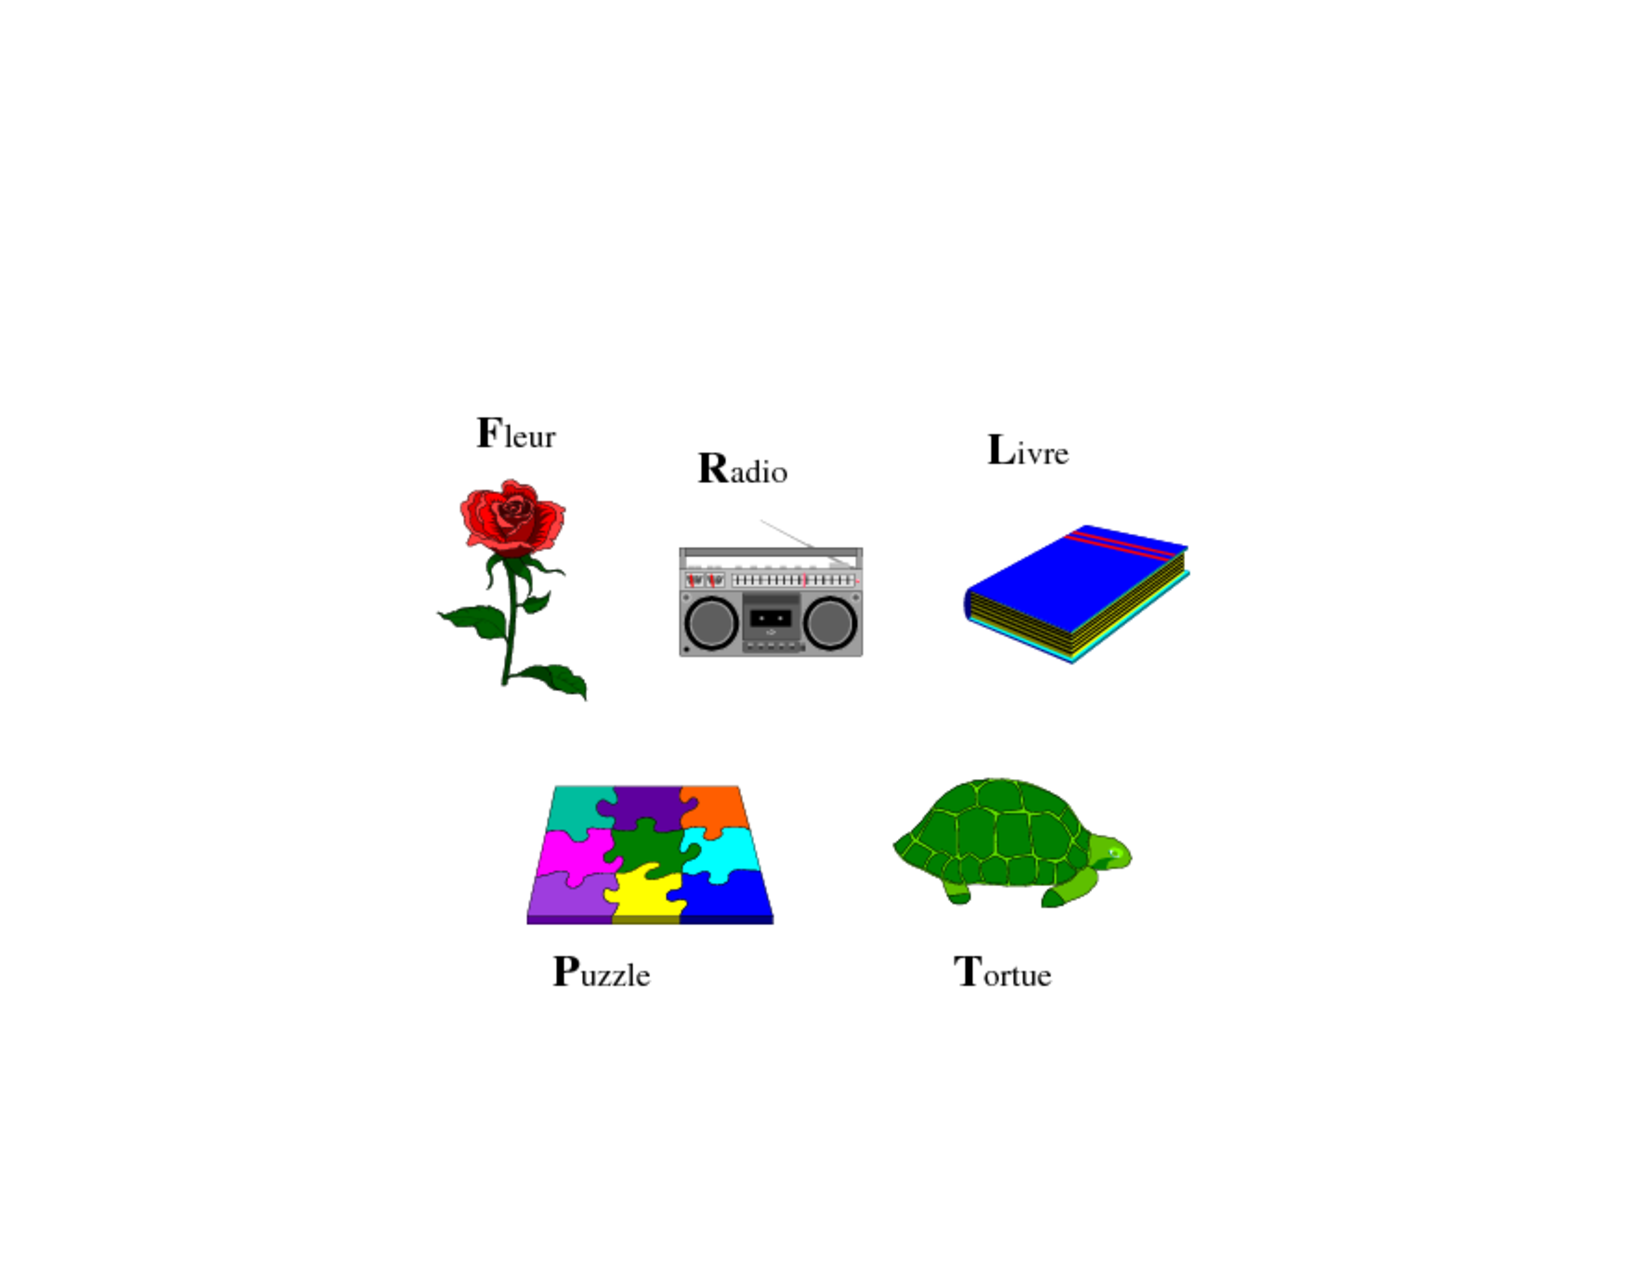
\includegraphics[width=0.4\textwidth,height=0.35\textheight]{gifts.pdf}
\end{figure}

\begin{figure}[h!]
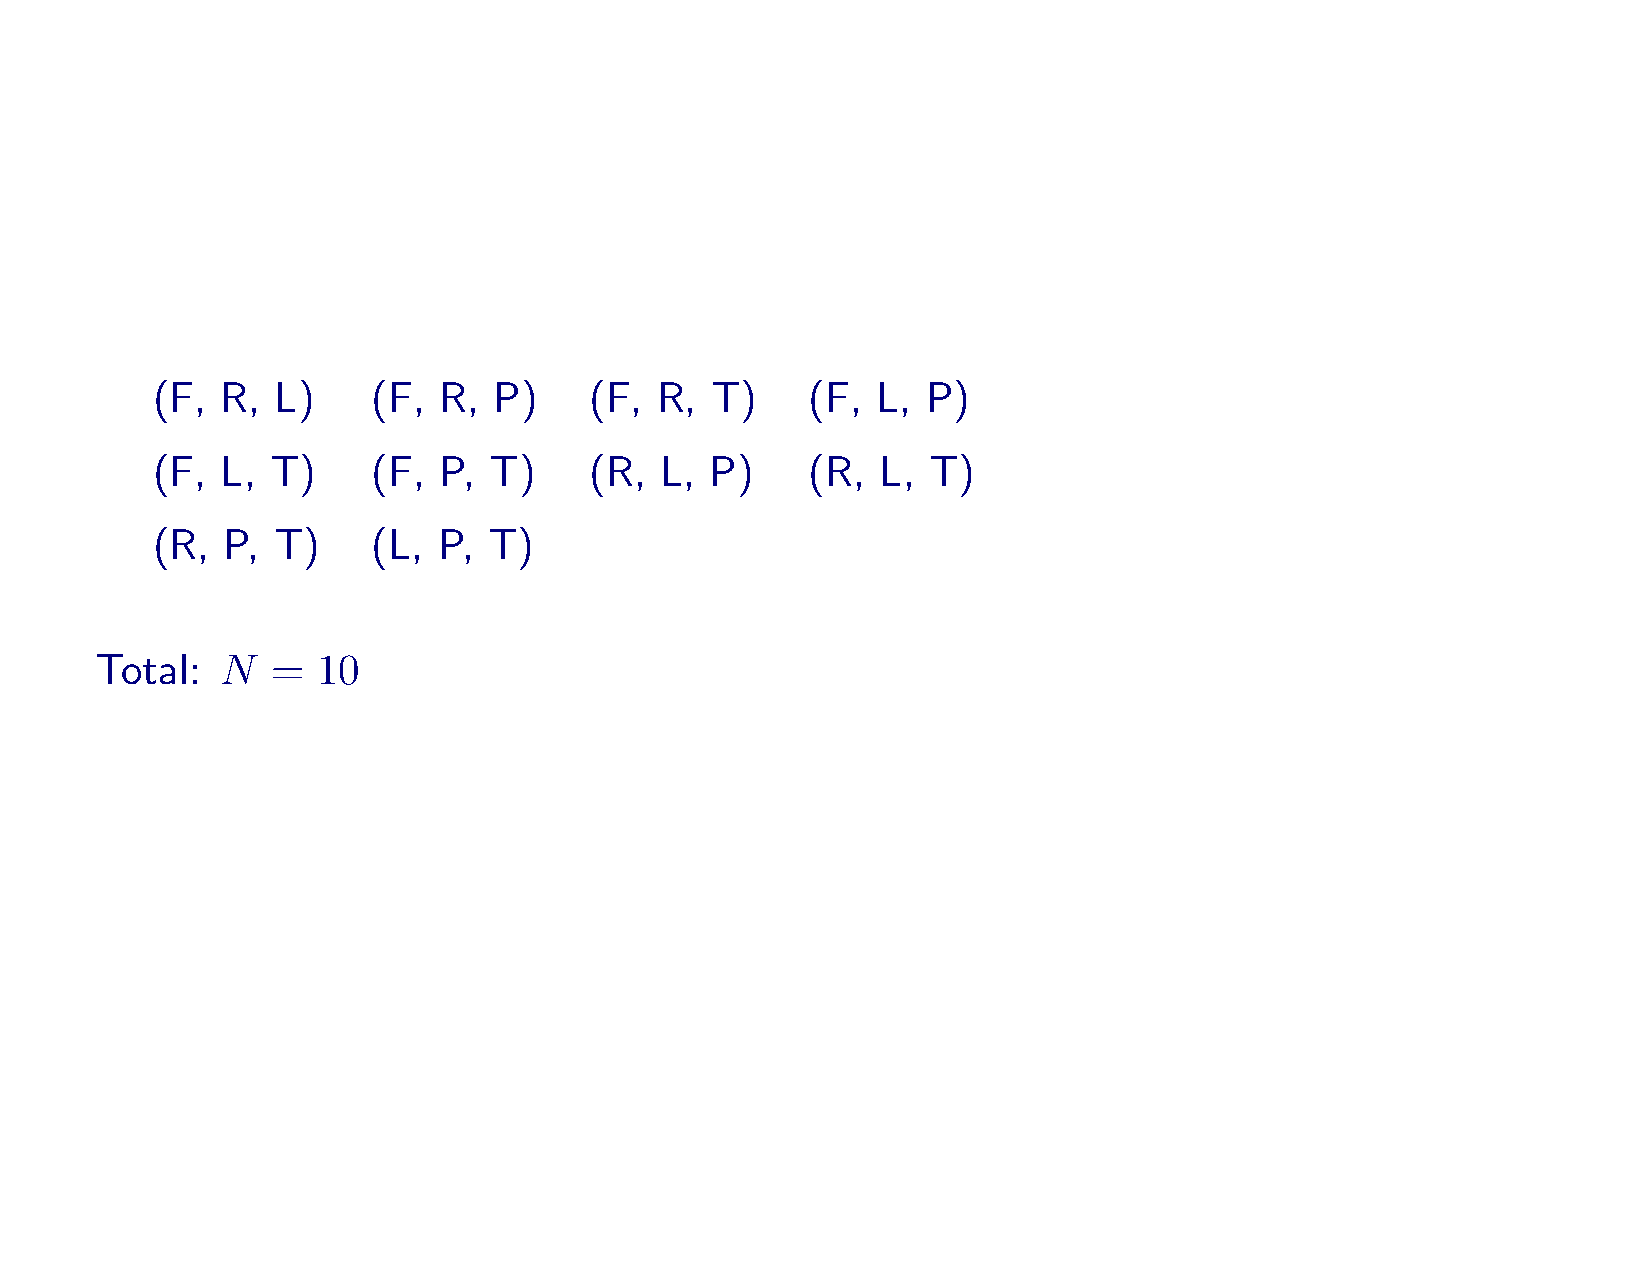
\includegraphics[width=0.5\textwidth,height=0.2\textheight]{outcomes.pdf}
\end{figure}
\end{example}

\end{frame}

\begin{frame}
\frametitle{Combinatorics}
\framesubtitle{An example}

\end{frame}


%\begin{frame}
%\frametitle{Some mathematical formulas (cont'd)}
%
%\begin{example}[cont'd]
%
%%How many ways can we select $3$ presents (order does not matter) among the $5$ available presents (see figure below)?
%
%\begin{figure}[h!]
%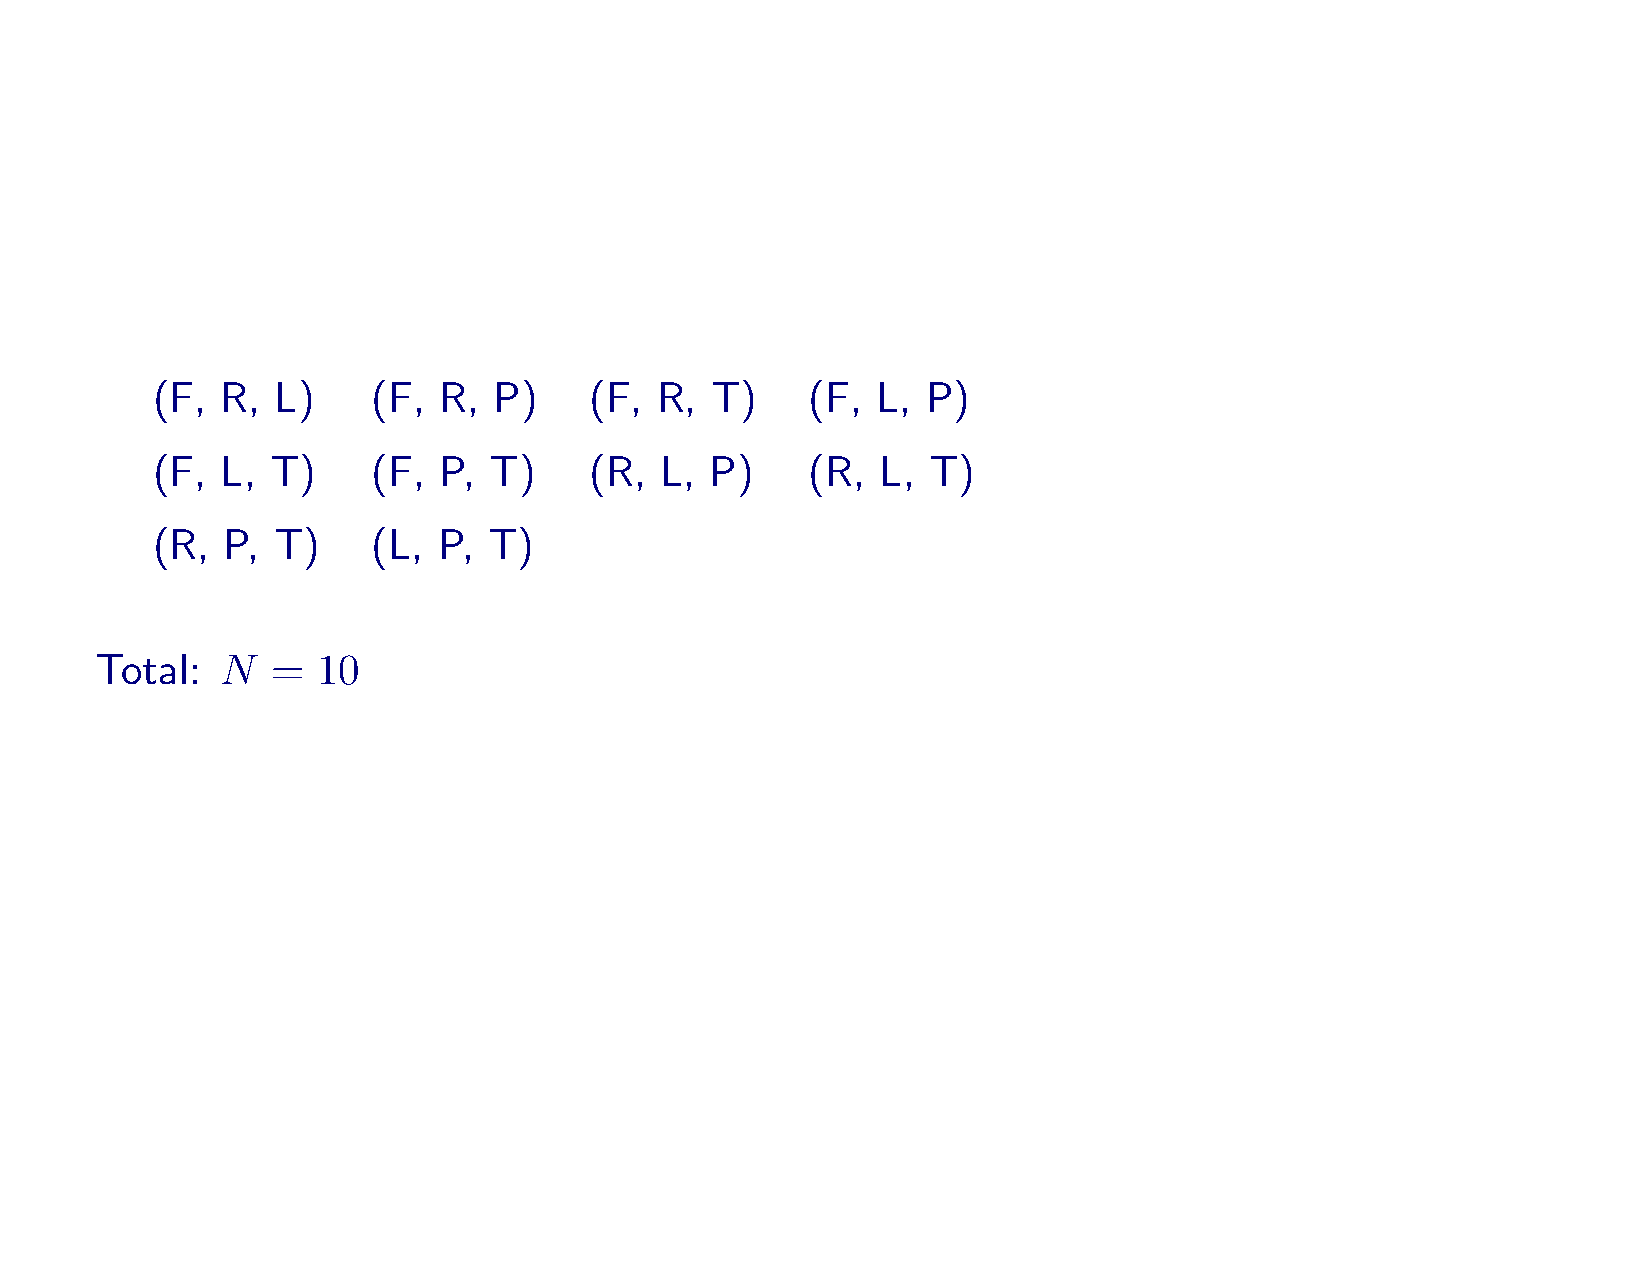
\includegraphics[width=0.6\textwidth,height=0.3\textheight]{outcomes.pdf}
%\end{figure}
%\end{example}
%
%\end{frame}

\begin{frame}
\frametitle{Combinatorics}
\framesubtitle{An example}
\begin{example}[Interpretation]
\begin{itemize}
\item[1] $5!$ gives you the total $\#$ permutations of the presents.
\item[2] Selecting $3$ presents implies \textbf{not selecting} $(5-3)$ other presents.
\begin{itemize}
\item Therefore, we need to divide or \textbf{"factor out"} the $(5-3)!$ permutations of the non-selected present  from the $5!$ permutations of all presents.
\end{itemize}
In other words you have $5! / (5-3) !$ ways to select and order the 3 presents;
\item[3] Finally, \textbf{we don't care about the order} of selection of the $3$ presents.
\begin{itemize}
\item All the permutations of this selection are deemed equivalent.
\item  e.g. (F, R,L ) is the same as (R, F, L)
\end{itemize}
Since there will be $3!$ permutations of the selection. This number needs to be \textbf{factored out}.
\end{itemize}
\end{example}

\end{frame}

\begin{frame}
\frametitle{Combinatorics}
\framesubtitle{An Example}
\begin{example}[continued]
... so, in formula, you have $$\frac{5!/(5-3)!}{3!}$$ ways to select the $3$ presents:
$$
\frac{5!/(5-3)!}{3!}= \frac{5!}{3!2!} = \binom 5 3 = C_5^3.
$$
This gives you the total $\#$ of possible ways to select the $3$ presents when the order does not matter.
\end{example}

As an exercise, redo the exercise assuming you can select 2 presents from 3 available presents
(like for instance F,L,R). Create all the combinations and then use the formulas to see how they coincide.

\end{frame}

\begin{frame}
\frametitle{Combinatorics}

\begin{remark}
\textbf{Combinations:} How many ways can we select $k$ objects among $n$?
\begin{enumerate}
\item How many ways can we combine $k$ objects among $n$?
\begin{itemize}
\item In the 1st place: $n$
\item In the 2nd place: $(n-1)$
\item ....
\item In the $k$-th place: $(n-k+1)$
\end{itemize}

\item We have $k!$ ways to permute the $k$ objects that we selected
\item The number of possibilities (without considering the order) is:
$$
\frac{n!/(n-k)!}{k!} = \frac{n!}{k!(n-k)!} \color{gray}{=C^{k}_n}\color{black}
$$
\end{enumerate}
\end{remark}

\end{frame}

\begin{frame}
\frametitle{Combinatorics}

\begin{remark} [cont'd]

In Problem Set $2$, you will have to make use of $C^{k}_n$ in Ex2-Ex3-Ex5.

Indeed, to compute the probability for an event $E$, will have to make use of the formula:

\begin{equation} \label{Eq: PE}
P(E)=\dfrac{\text{number of cases in E}}{\text{number of possible cases}}.
\end{equation}

This is a first intuitive definition of probability, which we will justify in the next lecture;

For the time being, let us say that the combinatorial calculus will be needed to express both the quantities (numerator and denominator) in (\ref{Eq: PE}).

\end{remark}

\end{frame}

\section{Limits}

\begin{frame}
\frametitle{Limits}

\begin{itemize}
\item The limit of a finite sum is an infinite series:
\bea
\lim_{n \to \infty} \sum_{i=1}^n x_i = \sum_{i=1 }^\infty x_i \nonumber
\eea
\item The $\exp()$ function, characterised as a limit:
\bea
%\lim_{x \to 0} \left(1+x\right)^{\frac{1}{x}} = \lim_{x \to \infty} \left(1+\frac{1}{x}\right)^{x} = e \nonumber
e^x = \lim_{n \rightarrow \infty} \left(1 + \frac{x}{n}\right)^n \nonumber
\eea
\item The Limit of a Negative Exponential function :
\bea
\text{for }\alpha >0, \ \  \lim_{x \to \infty} {\alpha e^{-\alpha x}} = 0 \nonumber
\eea
\item The Exponential function, characterised as an infinite series
\bea
e^x = \sum_{i = 0}^{\infty} {x^i \over i!} = 1 + x + {x^2 \over 2!} + {x^3 \over 3!} + {x^4 \over 4!} + \cdots \nonumber
\eea
\end{itemize}
\end{frame}


\begin{frame}
\frametitle{Wrap-up}


\textbf{Reminder of:}
\begin{itemize}
\item The power-to-$n$, $\exp()$ and $\ln()$ functions.
\item Elements of differential calculus (derivatives and integrals)
\item Sums, Double Sums
\item Limits
\end{itemize}
\pause

Most importantly, \textbf{Combinatorics}

\begin{itemize}
\item A set with $n$ elements has \textbf{$n!$ possible permutations}
\item There are $n!/(n-k)!$ ways of choosing $k$ elements from $n$ \textbf{when the order is important}
\item There are $n!/(k!(n-k)!)$ ways of choosing $k$ elements from $n$ \textbf{when the order is not important}
\end{itemize}


\begin{center}
In English, the symbol $\binom n k = C^n_k$ reads \textbf{"n choose k"}
\end{center}

\end{frame}

\begin{frame}
	\begin{center}

		\LARGE{Thank you for your attention!}

		\pause

		\LARGE{"See you" next week!}
	\end{center}
\end{frame}


\end{document}

